\section{Directed-Acyclic Graphs \& Topological Ordering}
Graphs may represent a variety of relationships, such as dependencies between tasks or the flow of information. 

\begin{Def}[Directed-Acyclic Graph (DAG)]
    
    A \textbf{directed-acyclic graph} is a directed graph with no cycles.
\end{Def}

\begin{figure}[h]
    \begin{center}
      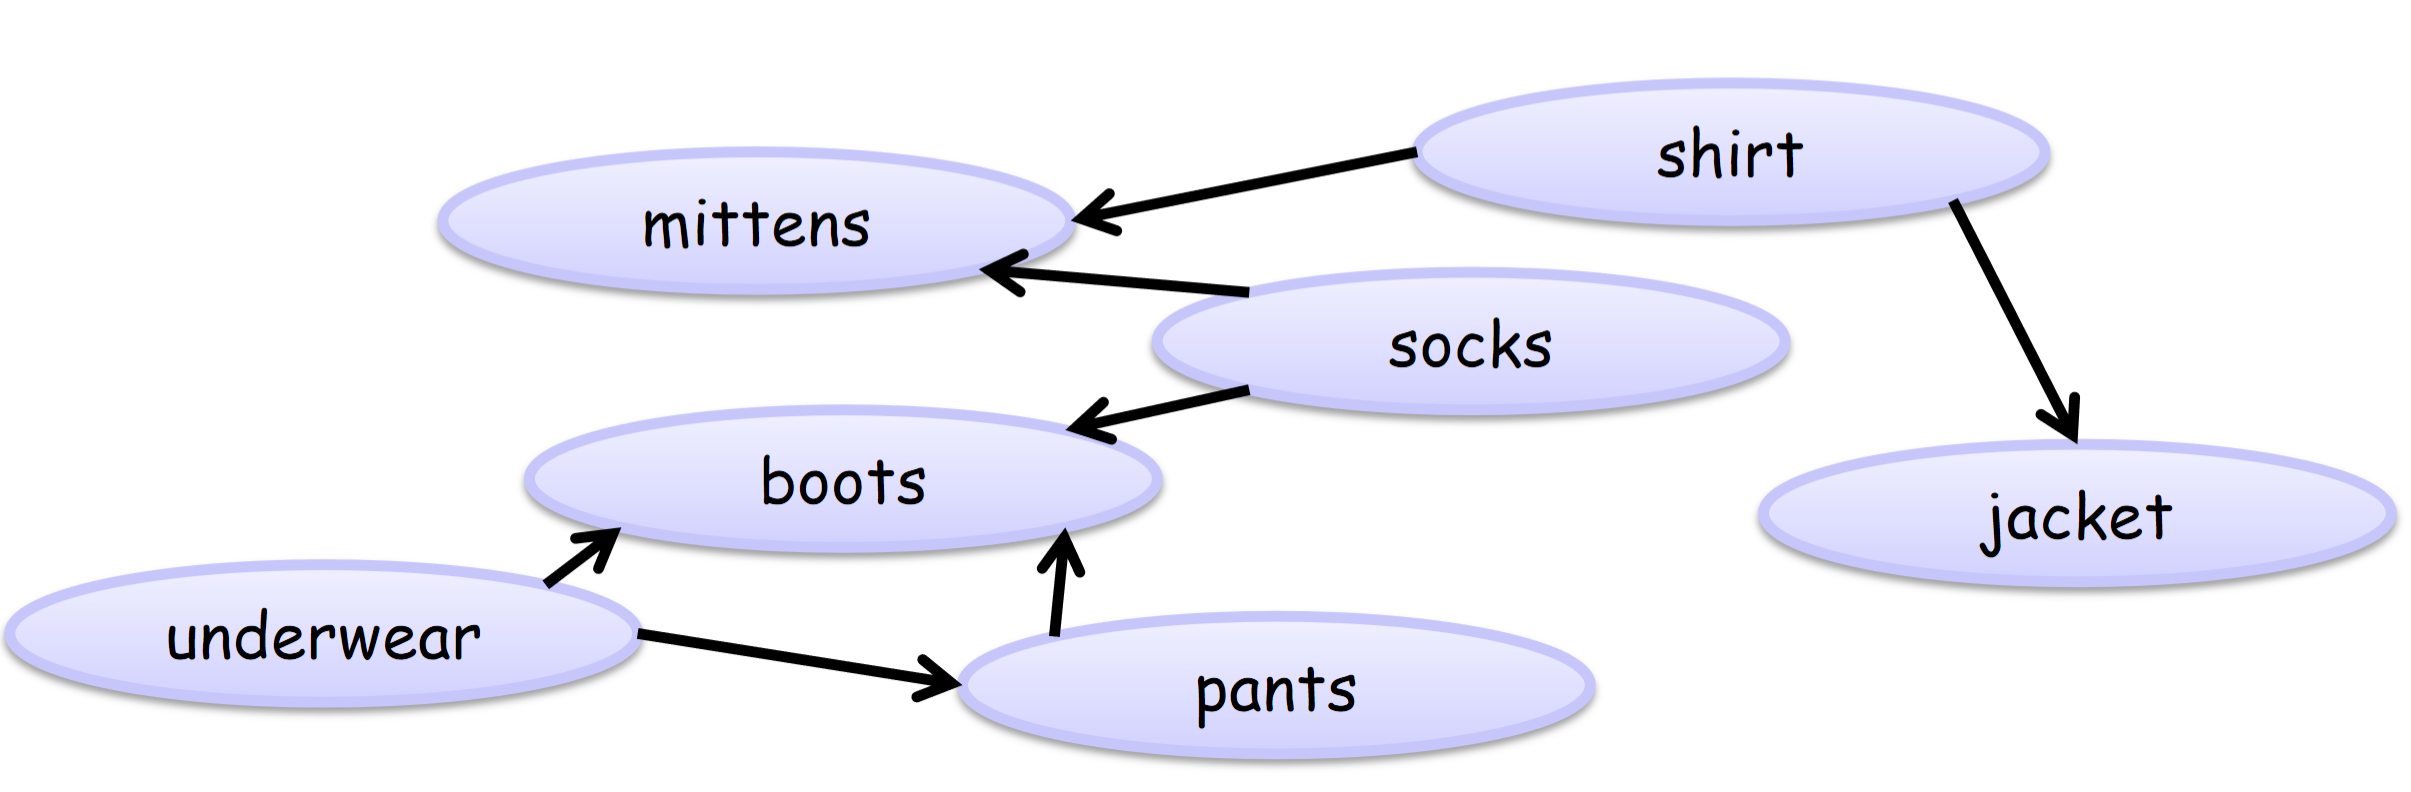
\includegraphics[height=1.5in]{./Sections/graphs/dag/dag.png}
    \end{center}
     \caption{A DAG depicted by getting dressed for winter. For each node to be processed its \textbf{dependencies} or parents must be processed first.}\label{fig:dag}
\end{figure}

\noindent


\begin{Def}[Topological Ordering]

    Given a graph, a \textbf{topological ordering} is a linear ordering of nodes such that for every edge $(u,v)$, $u$ comes before $v$.
\end{Def}

\begin{figure}[h]
    \begin{center}
      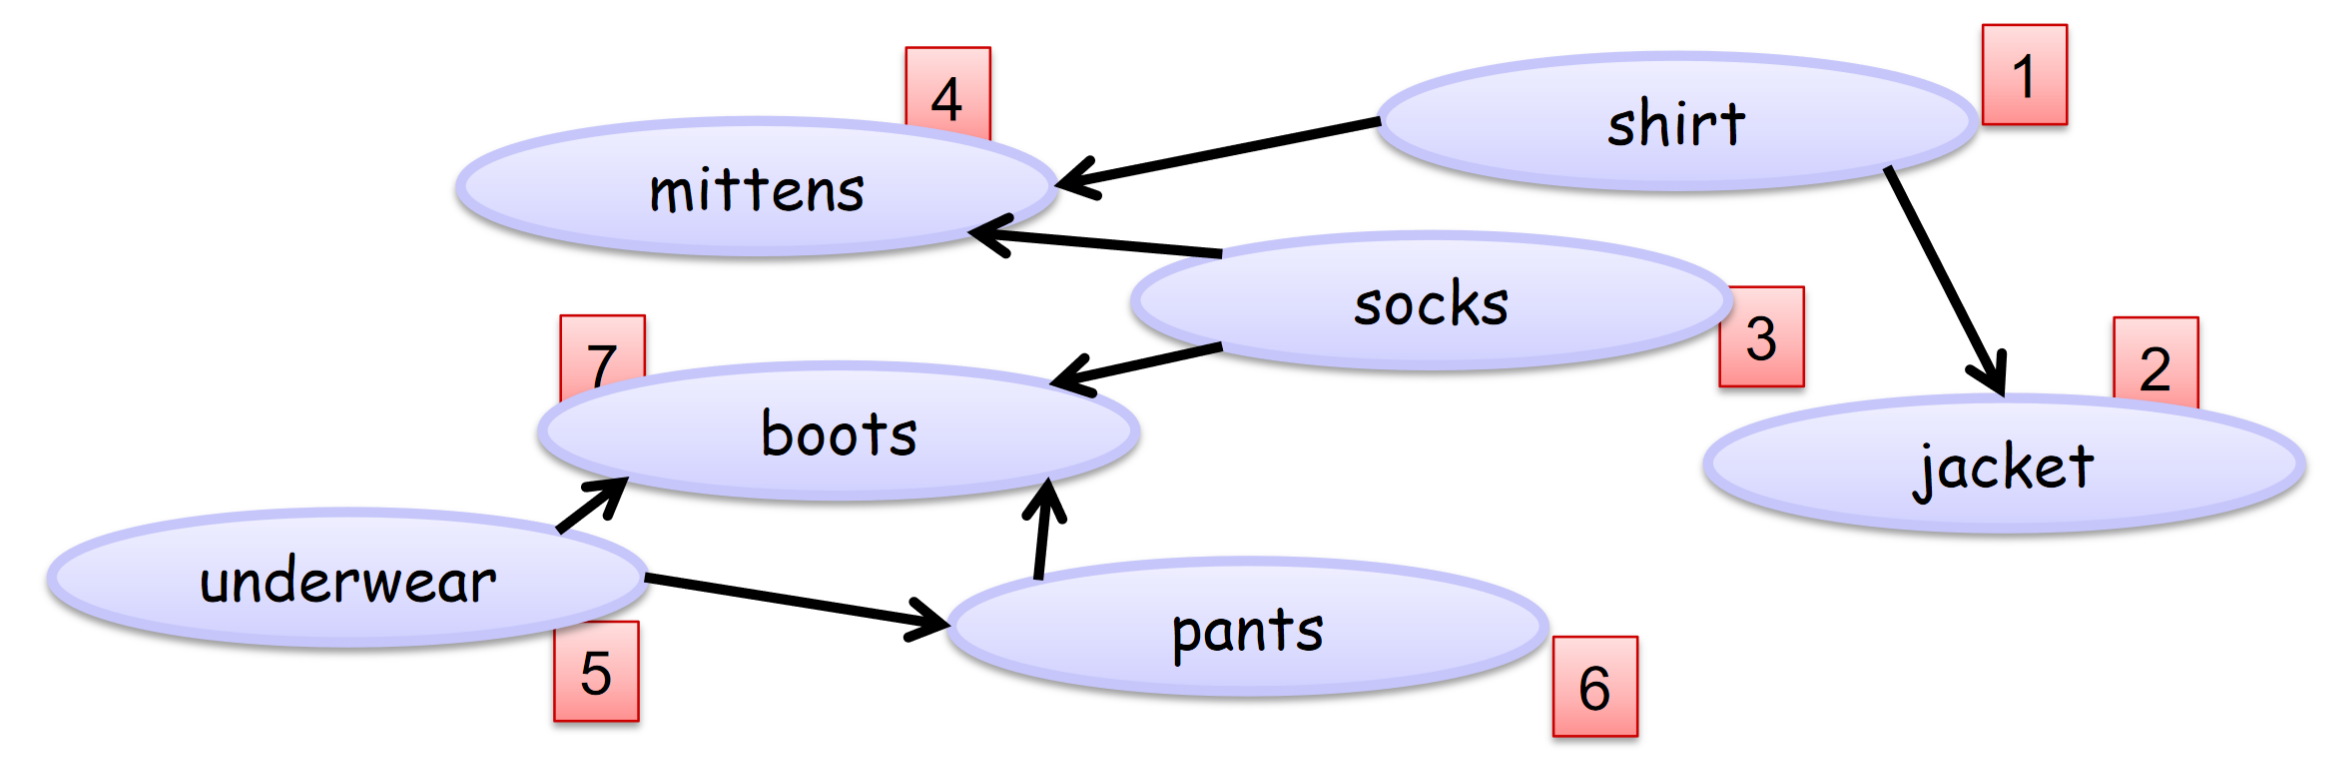
\includegraphics[height=1.5in]{./Sections/graphs/dag/top.png}
    \end{center}
     \caption{A topological ordering of the DAG in Figure (\ref{fig:dag}) enumerated in red.
     Another possible ordering of $[1,2,3,4,5,6,7]$ is $[5, 6,1,2,3,4,7]$, as $5\rightarrow 6$ is independent.}\label{fig:top}
\end{figure}
\noindent

\newpage 
\begin{theo}[Topological Sort]
    
    Given a DAG, a topological ordering can be found.
\end{theo}
\begin{figure}[h]
    \begin{center}
      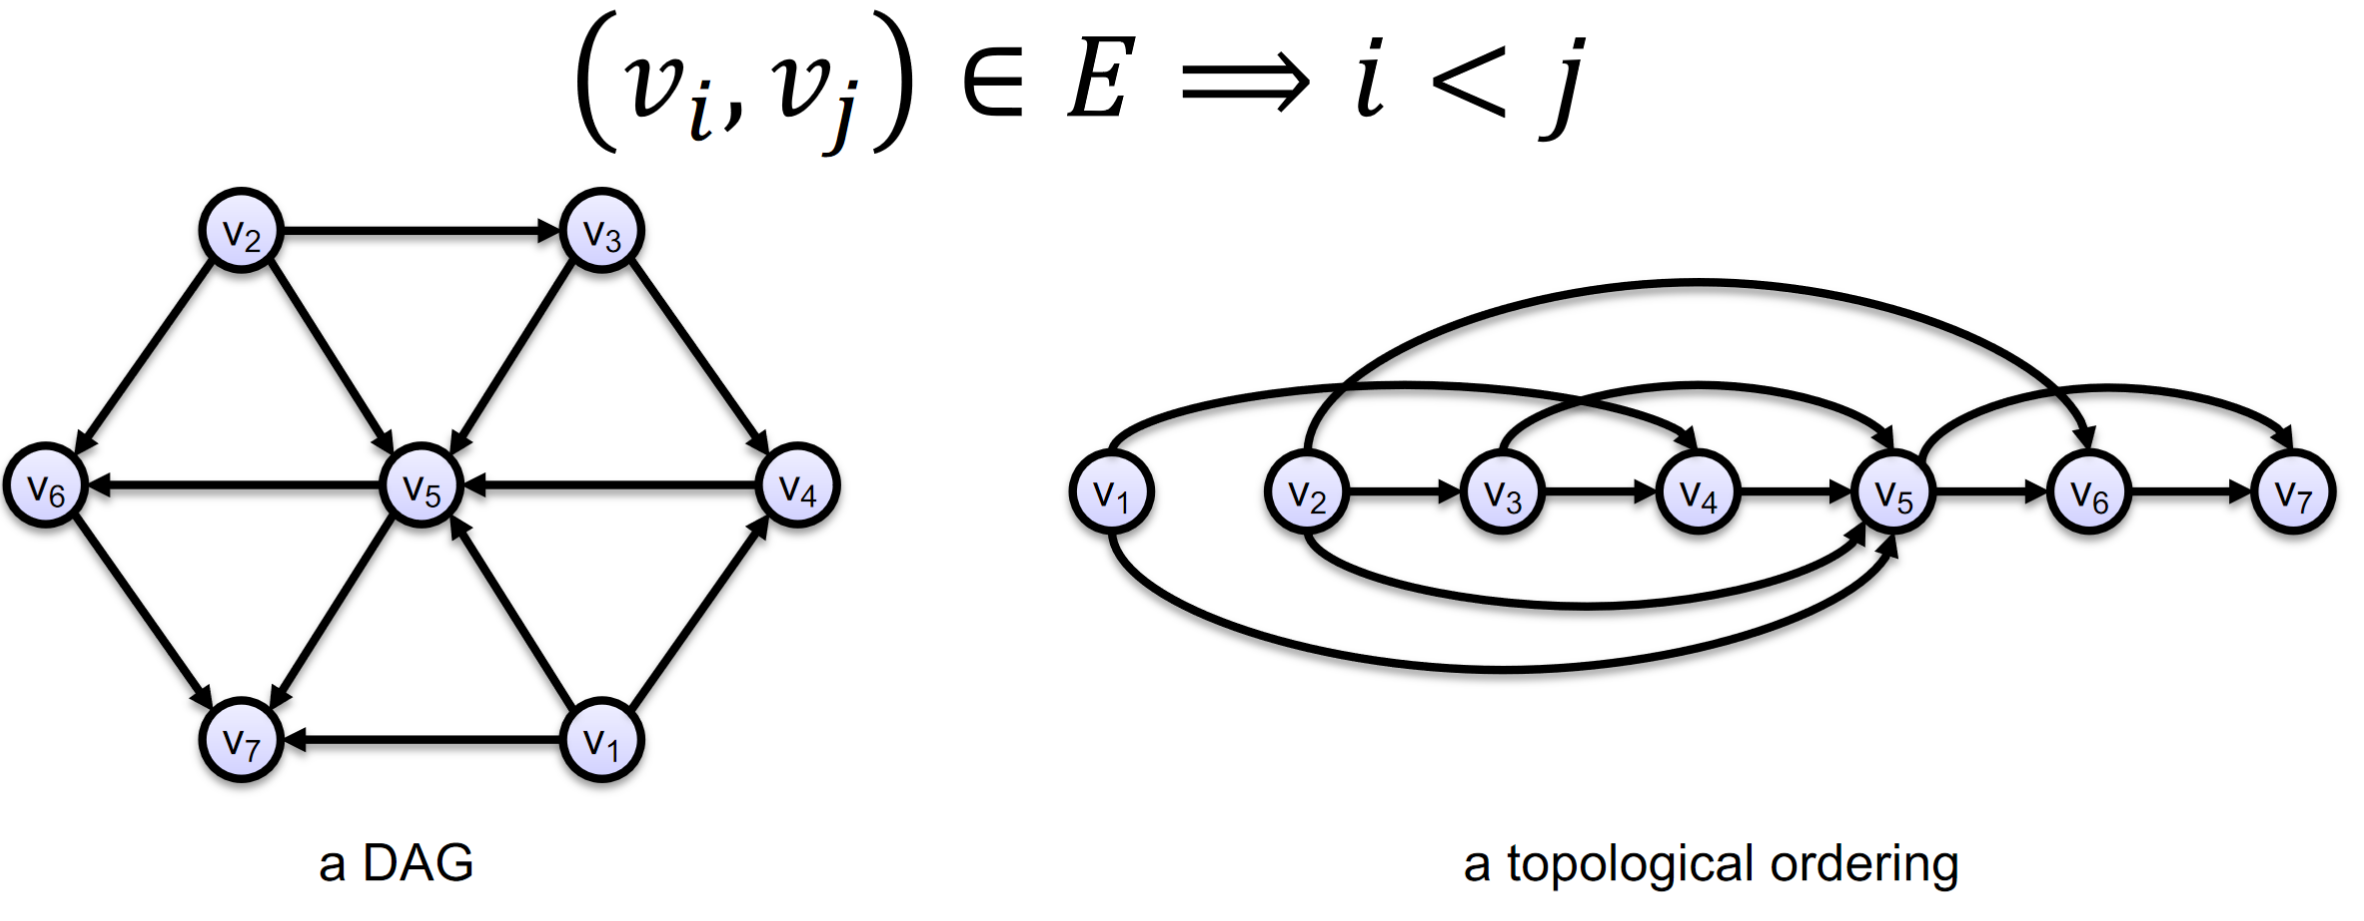
\includegraphics[height=2.5in]{./Sections/graphs/dag/top_sort.png}
    \end{center}
     \caption{A topological sorting of a DAG $E$ and $v$ nodes}\label{fig:top_sort}
\end{figure} 

\begin{Proof}[Topological Sort via DFS]
    \textit{\textbf{Lemma:}} In a directed graph $G$, if (note necessarily acyclic):
    \begin{itemize}
        \item $(u, v)$ is an edge, and
        \item $v$ is not reachable from $u$,
    \end{itemize}
    Then in every run of DFS, $u.f > v.f$.
    
    \noindent
    \textit{\textbf{Proof:}}
    \begin{itemize}
        \item If $v$ is started before $u$, then the DFS-Visit($v$) will terminate without reaching $u$ (because there is no path to $u$).
        \item If $u$ is started before $v$, then the edge $(u, v)$ will be explored before $u$ is finished.
    \end{itemize}
    Therefore, in all cases, $u.f > v.f$.
\end{Proof}

\newpage 

\begin{Def}[Strongly Connected Components]

    A \textbf{strongly connected component} is a subgraph where every node is reachable from every other node. 
    Then we say $u\rightsquigarrow v$ and $v\rightsquigarrow u$ are \textbf{mutually reachable}. 
\end{Def}

\vspace{3em}
\begin{figure}[h]
    \begin{center}
      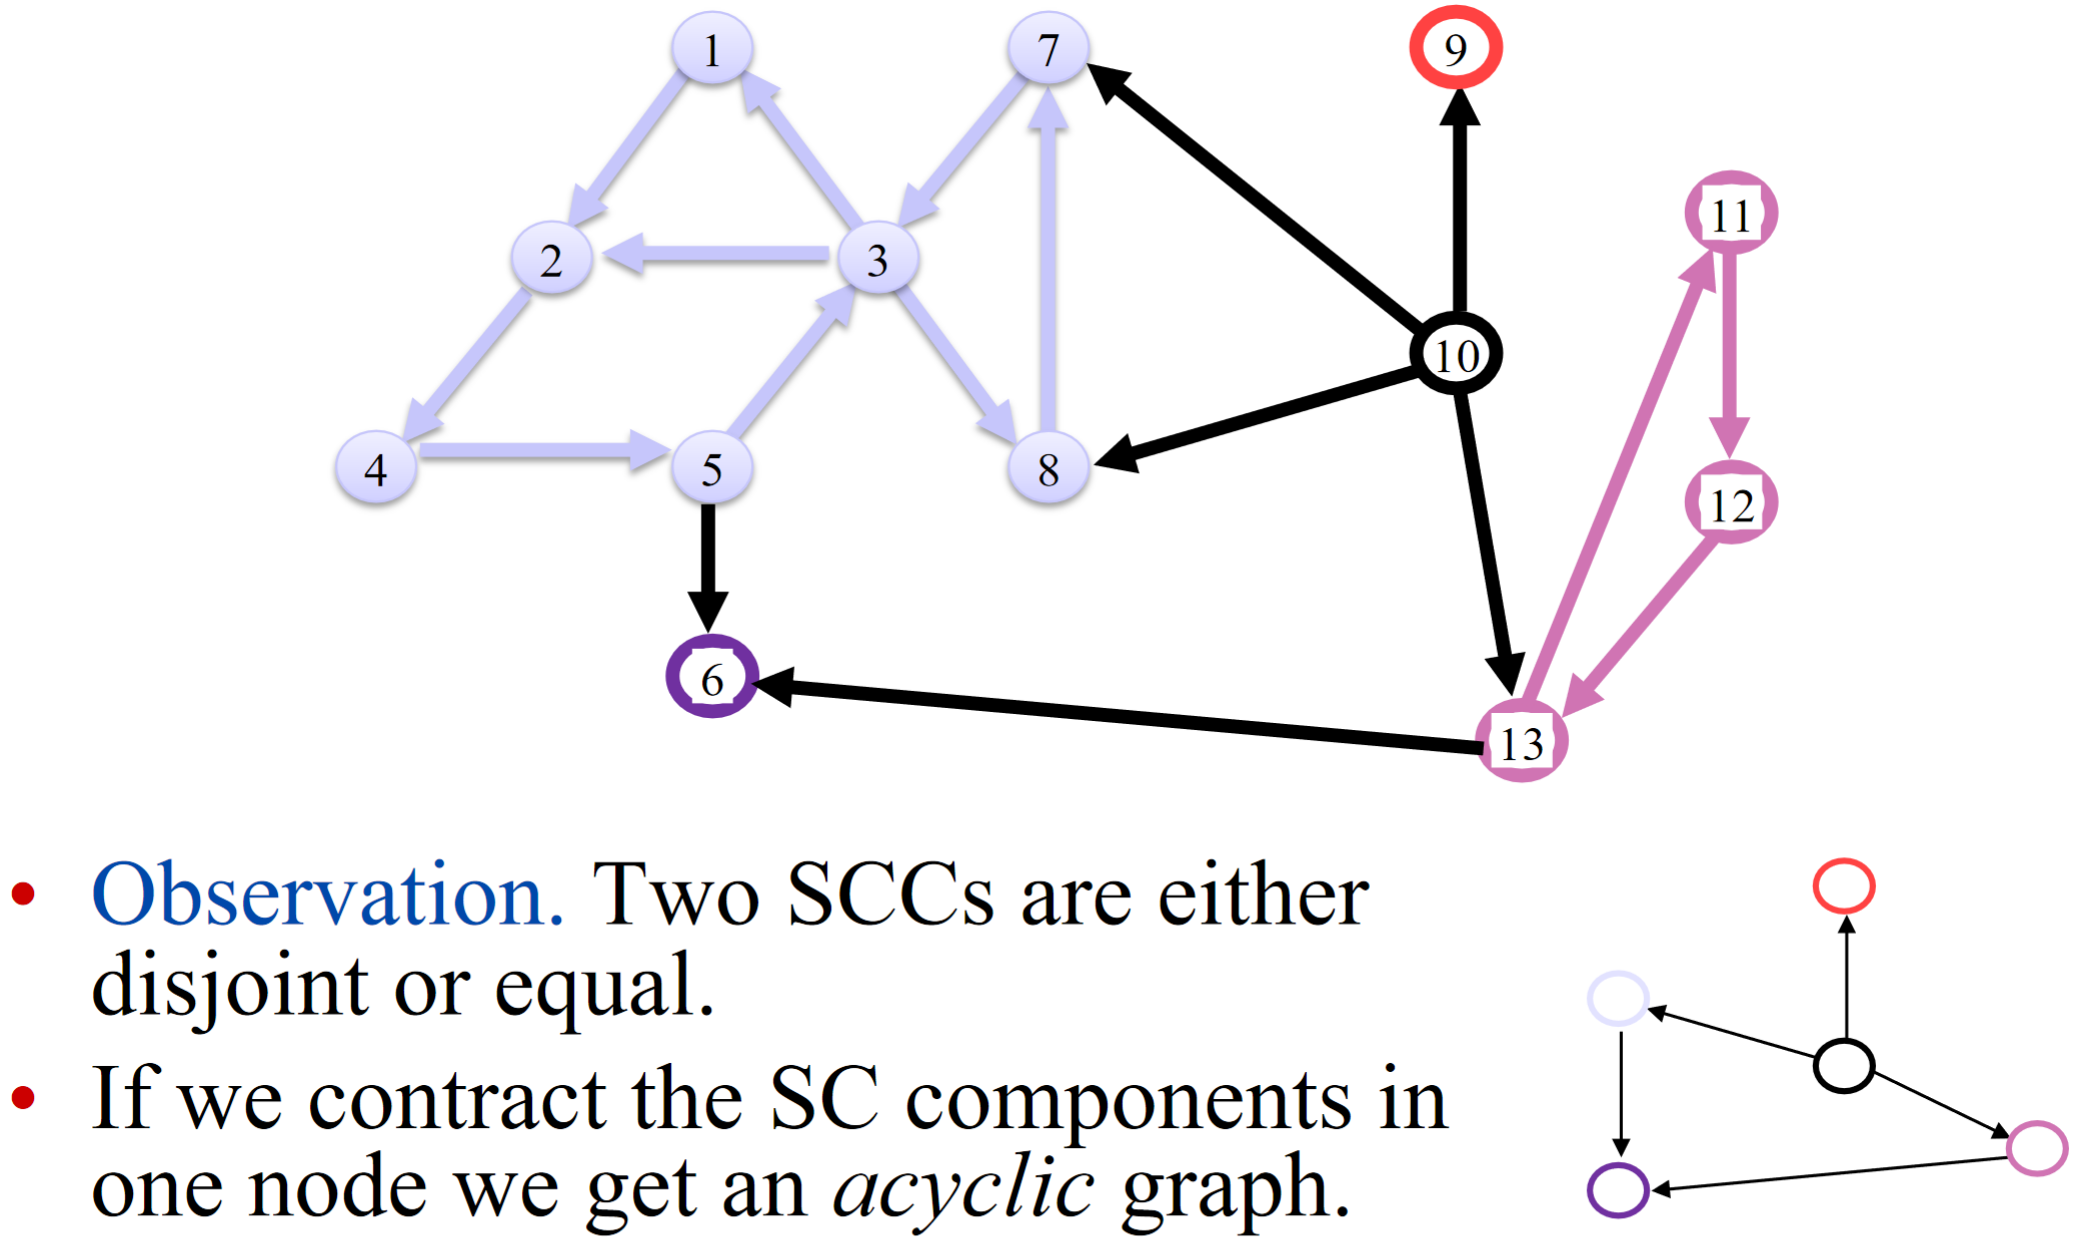
\includegraphics[height=3.4in]{./Sections/graphs/dag/strong_conn.png}
    \end{center}
     \caption{A graph with 5 strongly connected components.}\label{fig:strong_conn}
\end{figure}

\newpage 

\begin{Exercise}Based on the images which are trees, and if not, why?

    \label{ex:tree}
    \vspace{1em}
    \hspace{-2em}
    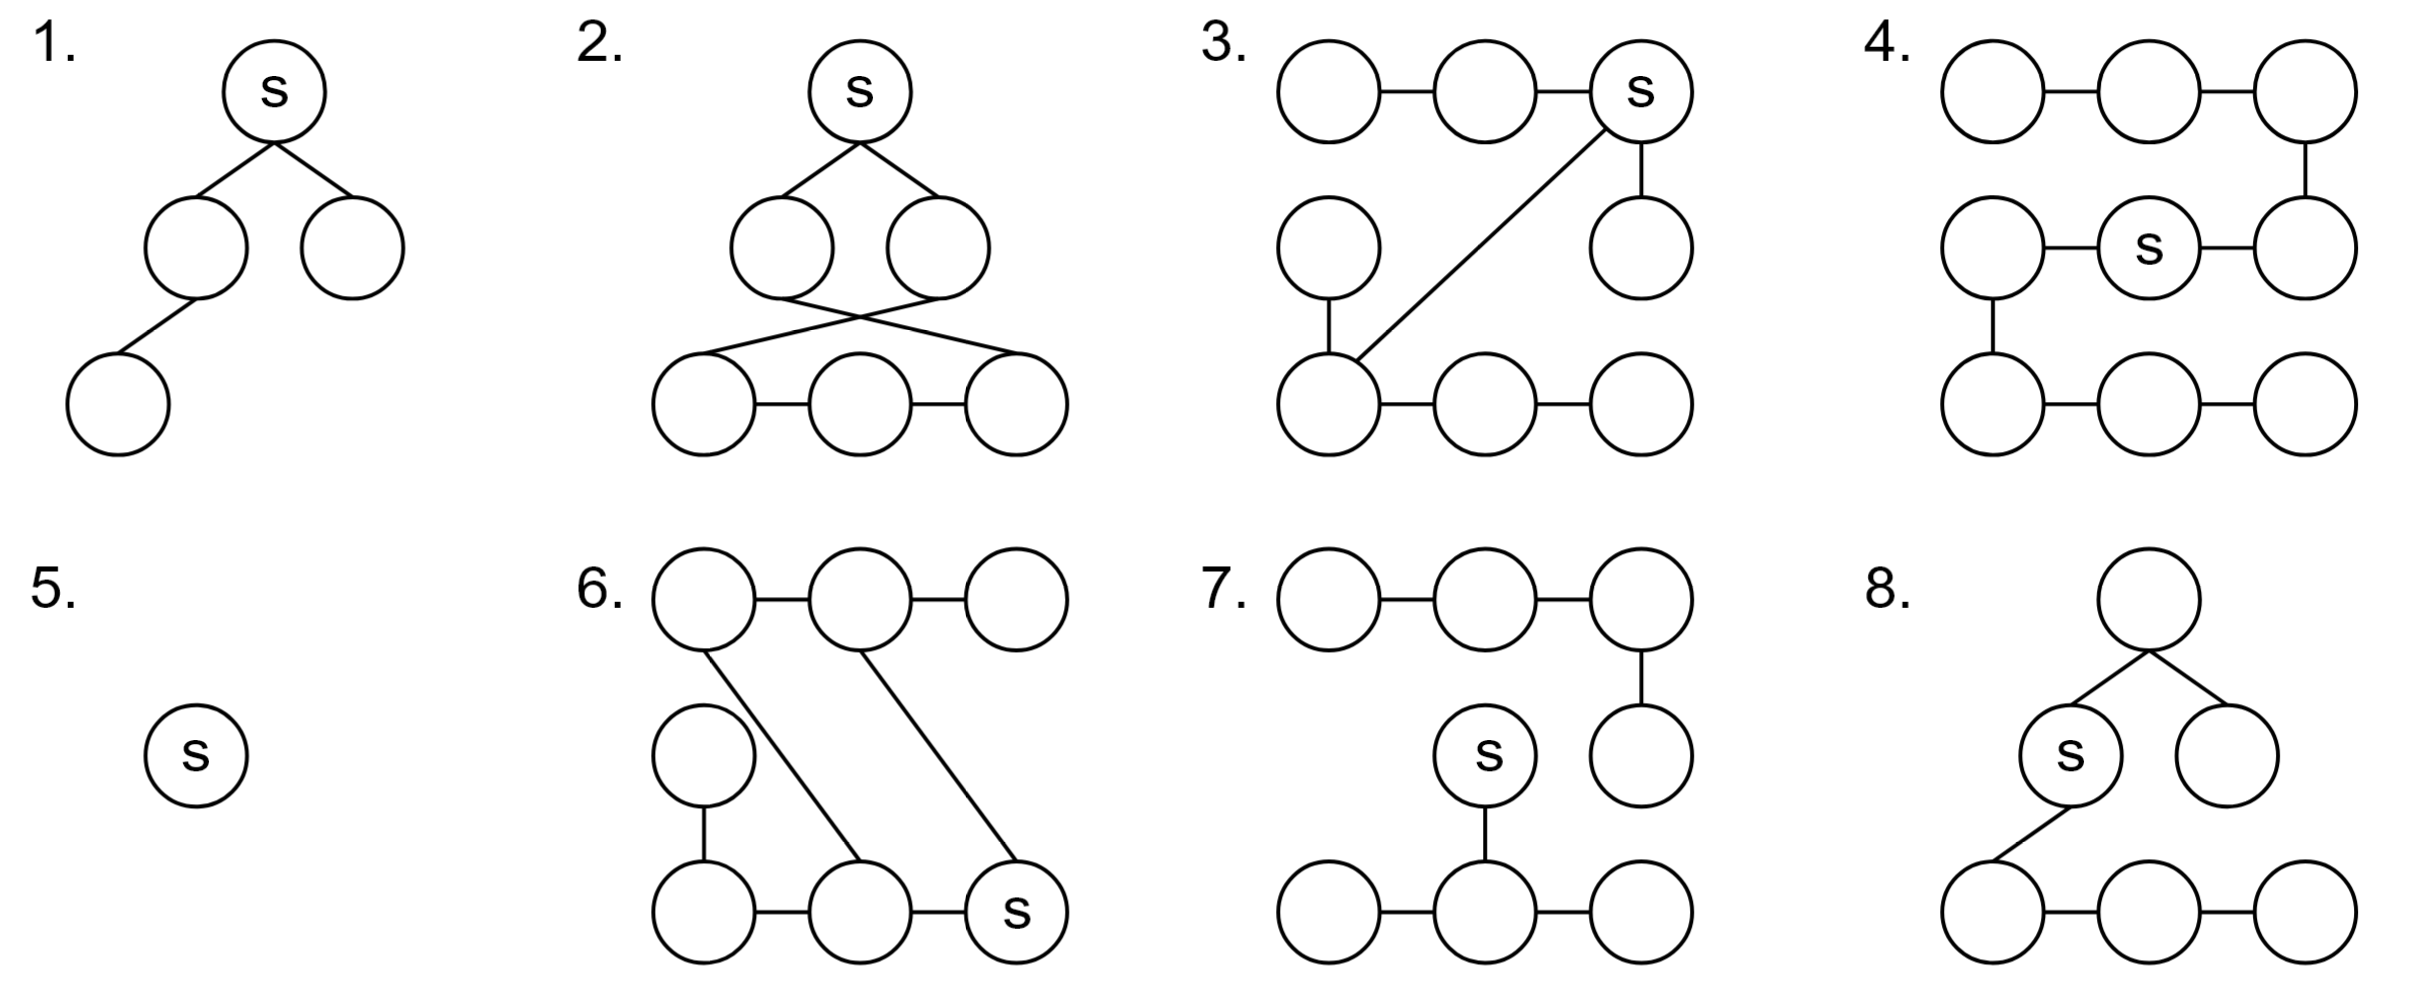
\includegraphics[height=2.4in]{./Sections/graphs/dag/tree_example.png}

\end{Exercise}

\begin{Exercise} Based on Exercise (\ref{ex:tree}) above, starting with the $s$ nodes,
    what are possible results of BFS and DFS?
\end{Exercise}

\vspace{.5em}
\begin{Exercise} What type of edges do BFS and DFS traversals produce on directed and undirected graphs?
\end{Exercise}

\vspace{.5em}
\begin{Exercise} BFS can find shortest paths, does DFS find longest paths (True/False)?
\end{Exercise}

\vspace{.5em}
\begin{Exercise} To find a path and return such path from node $s$ to node $t$ in a graph, should we use 
    BFS or DFS?
\end{Exercise}

\vspace{.5em}
\begin{Exercise} To detect cycles in a graph, should we use BFS or DFS, or both?
\end{Exercise}

\vspace{.5em}
\begin{Exercise} Say we wanted to find the shortest round-trip path, that is, the minimal path starting from origin node $s$ visiting a set of
    nodes exactly once returning to $s$. How should we use BFS or DFS?
\end{Exercise}

\vspace{.5em}
\begin{Exercise} Which of the below images are DAGs.

    \label{ex:dag}
    \vspace{1em}
    \hspace{-2em}
    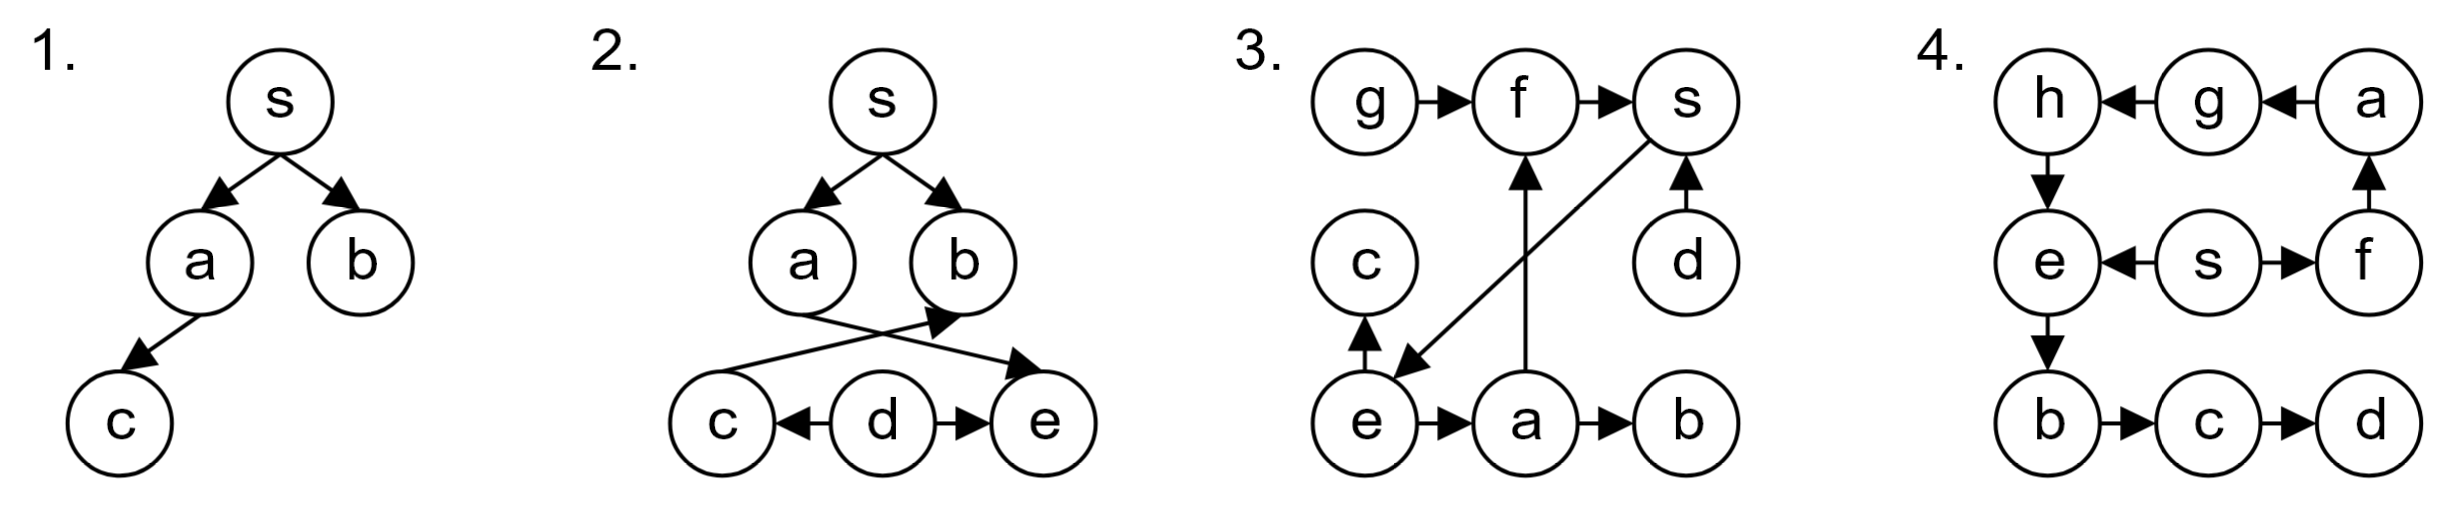
\includegraphics[height=1.2in]{./Sections/graphs/dag/dag_example.png}
\end{Exercise}

\vspace{.5em}
\begin{Exercise} Based on Exercise (\ref{ex:dag}) above, what are possible topological orderings?
\end{Exercise}

\newpage 

\begin{Answer} 1, 3, 4, 5, 8 are trees. 2 has a cycle, 6 has a cycle, 7 is disconnected.
\end{Answer}
\begin{Answer} There are other possible solutions depending on order of traversal. For 7,
    BFS and DFS don't alone handle disconnected graphs. Though modifications could be made to handle such.
    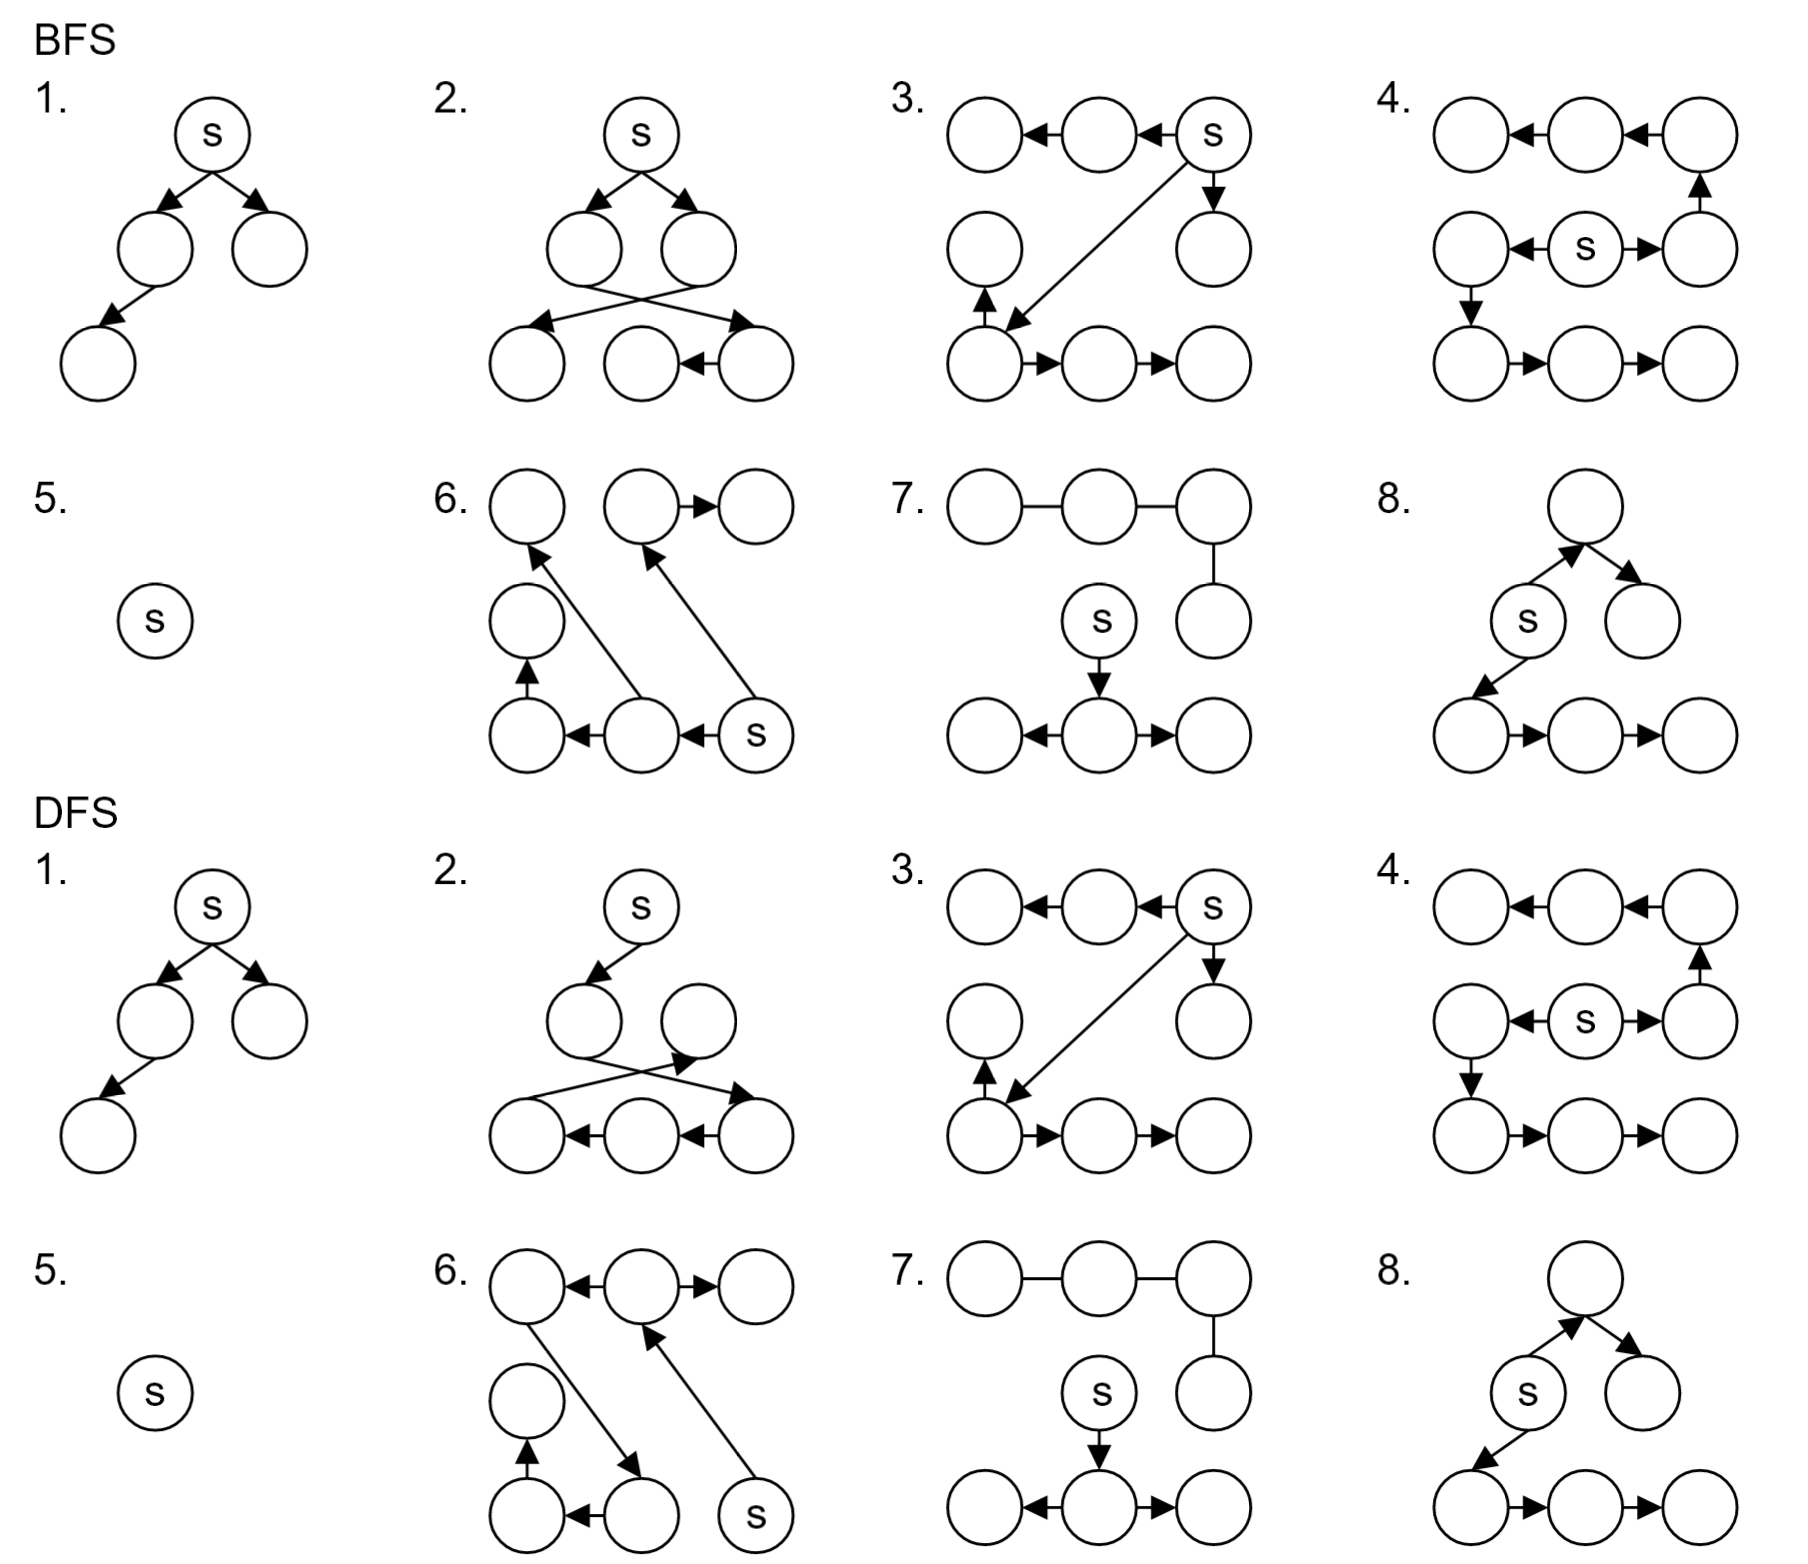
\includegraphics[height=4in]{./Sections/graphs/dag/bfs_dfs.png}
\end{Answer}

\vspace{.5em}
\begin{Answer} Undirected - BFS: Tree edges, DFS: Tree edges, Back edges. Directed - BFS: Tree edges, Back edges, Cross edges, DFS: Tree edges, Back edges, Forward edges, Cross edges \cite{cse417dfs2021,dukegraph2017,clrs22-1}
\end{Answer}

\vspace{.5em}
\begin{Answer} False, as of today, there is no known algorithm to find the longest path in a graph.
\end{Answer}

\vspace{.5em}
\begin{Answer} BFS, it finds shortest child-parent connections, giving us a direct path from $s$ to $t$.
\end{Answer}

\vspace{.5em}
\begin{Answer} Both, as DFS when it encounters a node that has already been visited, it has found a cycle. BFS when two branches meet, a cycle is found.
\end{Answer}

\vspace{.5em}
\begin{Answer} BFS, one implementation is to run BFS from $s$ to all nodes, the first cycle found is the shortest round-trip path.
\end{Answer}

\vspace{.5em}
\begin{Answer} 1, 2, and 4 are DAGs. 3 has a cycle (f,s,e,a).
\end{Answer}

\vspace{.5em}
\begin{Answer} 
    \begin{itemize}
        \item[1.] $[s,a,b,c]$, $[s,b,a,c]$, $[s,a,c,b]$. 
        \item[2.] $[s,a,d,c,b,e]$, $[d,c,s,a,e,b]$ or $[d,c,s,a,b,e]$
        \item[4.] $[s,f,a,g,h,e,b,c,d]$ 
    \end{itemize}
\end{Answer}

